\documentclass{article}
\usepackage[left=2cm, right=2cm]{geometry}
\usepackage{multicol}
\usepackage{graphicx}
\usepackage{subcaption}
\usepackage{listings}

\setlength{\columnsep}{1.5cm}

\lstdefinestyle{mystyle}{
    basicstyle=\footnotesize,
    breakatwhitespace=false,
    breaklines=true,            
    tabsize=1,
    frame=single
}
 
\lstset{style=mystyle}

\title{
    \textbf{Programação 3D} \\
    Relatório Técnico da Primeira Entrega
}
\author{Afonso Mercier \and Pedro Quintas \and Pedro Caldeira}
\date{}

\begin{document}
    \maketitle

    \begin{multicols}{2}
    \section{Funcionamento do Programa}

    O trabalho desenvolvido consiste numa aplicação de ray tracing na linguagem
    C++. O programa pode ser configurado para ler um ficheiro NFF e produz uma
    imagem fotorrealista com base na cena descrita no ficheiro. \\
    O desenvolvimento focou-se nos seguintes aspetos:

    \begin{itemize}
        \item Leitura de ficheiros NFF.
        \item Cálculo dos Raios Primários
        \item Cálculo da componente local da cor.
        \item Suporte para multiplas fontes luminosas.
        \item Sombras de contorno rígido.
        \item Reflecção de raios.
        \item Refracção de raios.
        \item Intersecções de raios com algumas primitivas.
        \begin{itemize}
            \item Esferas
            \item Planos Infinitos
            \item Triângulos
            \item AABBs
        \end{itemize}
    \end{itemize}

    \section{Leitura de Ficheiros NFF}
    
    Ipsum Lorem

    \section{Raios Primários}

    Ipsum Lorem

    \section{Componente Local da Cor}

    Ipsum Lorem

    \section{Fontes Luminosas}

    Ipsum Lorem

    \section{Sombras}

    Ipsum Lorem

    \section{Reflecção}

    Quando um raio intersecta um objecto, caso a componente especular do material
    seja superior a zero, é necessário calcular a cor relativa à reflecção da
    cena no objecto. Este calculo é feito através de uma chamada recursiva à função
    \verb|rayTracing| utilizando um novo raio. O novo raio é calculado de modo
    a fazer um ângulo com a normal na colisão igual ao ângulo entre o raio incidente
    e a normal na colisão. \\
    A cor resultante desta reflecção é atenuada de acordo com a componente especular
    do material do objeto.

    \begin{lstlisting}[language=C++]
if (col.object->_matProps->specularComp > 0 && depth < DEPTH_TRACE_LIMIT) {
    Ray reflector;
    reflector.versor = normalize(subVector(ray.versor, vector3MultScalar(col.normal, 2 * internalProduct(ray.versor, col.normal))));
    reflector.origin = addVector(col.point, vector3MultScalar(reflector.versor, EPSILON));

    Color reflected = colorTimesConstant(rayTracing(reflector, depth + 1, RefrIndex), col.object->_matProps->specularComp);
    color = addColors(color, reflected);
}
    \end{lstlisting}

    O raio criado é ligeiramente deslocado, de modo a evitar intersecções com o objecto reflector. Dada a natureza recursiva do algoritmo de \textit{Ray Tracing} é necessário
    limitar a profundidade que o algoritmo pode alcançar.

    \section{Refracção}

    Quando um raio intersecta um objecto translúcido a sua direcção é alterada
    de acordo com a lei de Snell. Visto que um raio tem uma direcção única, é criado
    um novo raio e a cor resultante deste raio é atenuada de acordo com
    a transmitância do objecto. A direcção do novo raio é resultante da aplicação
    da lei de Snell, $\eta_1/\eta_2 = sin(\theta_1)/sin(\theta_2)$.

    \section{Intersecções}

    Ipsum Lorem

    \subsection{Esferas}

    Ipsum Lorem

    \subsection{Planos Infinitos}

    Ipsum Lorem

    \subsection{Triângulos}

    Ipsum Lorem

    \subsection{AABBs}

    Ipsum Lorem

    \end{multicols}

    \newpage
    \section{Imagens}

    \begin{figure}[h!]
        \centering
        \begin{subfigure}{.2\linewidth}
            \centering
            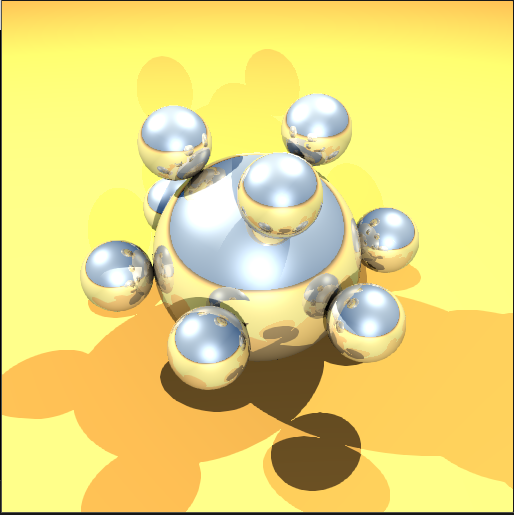
\includegraphics[width=\linewidth]{balls_low.png}
            \caption{balls\_low.nff}
            \label{fig:balls_low}
        \end{subfigure}
        \begin{subfigure}{.2\textwidth}
            \centering
            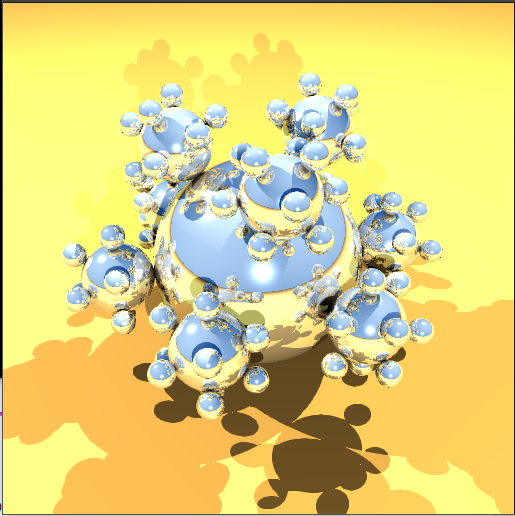
\includegraphics[width=\linewidth]{balls_medium.png}
            \caption{balls\_medium.nff}
            \label{fig:balls_medium}
        \end{subfigure}
        \begin{subfigure}{.2\linewidth}
            \centering
            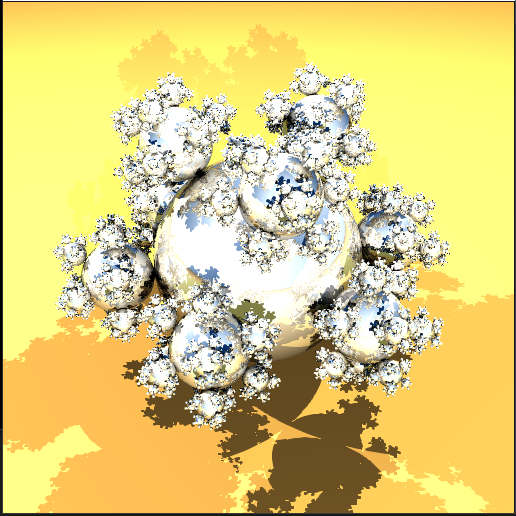
\includegraphics[width=\linewidth]{balls_high.png}
            \caption{balls\_high.nff}
            \label{fig:balls_high}
        \end{subfigure}

        \caption{Reflecções}
        \label{fig:balls}
    \end{figure}

    \begin{figure}[h!]
        \centering
        \begin{subfigure}[b]{.2\linewidth}
            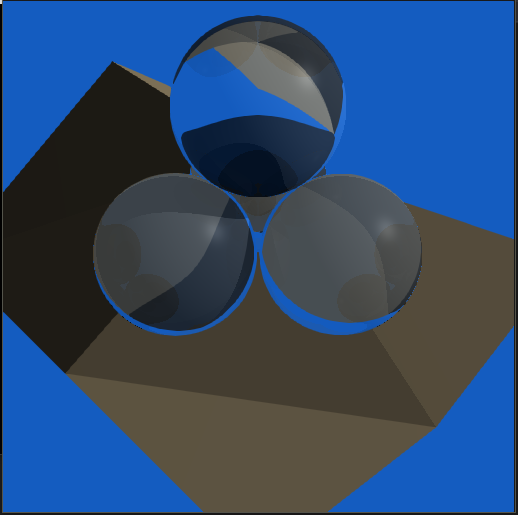
\includegraphics[width=\linewidth]{mount_low.png}
            \caption{mount\_low.nff}
            \label{fig:mount_low}
        \end{subfigure}
        \begin{subfigure}[b]{.2\linewidth}
            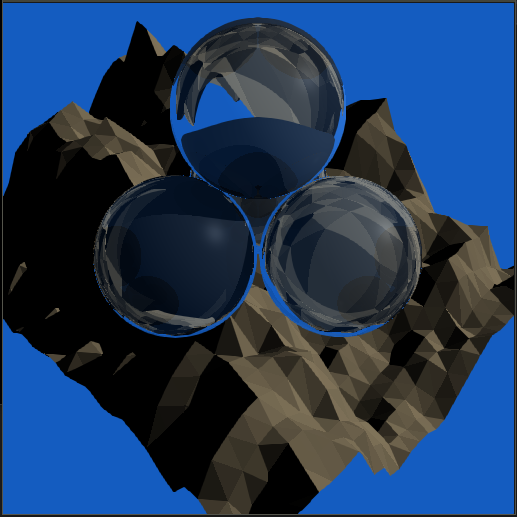
\includegraphics[width=\linewidth]{mount_high.png}
            \caption{mount\_high.nff}
            \label{fig:mount_high}
        \end{subfigure}
        \begin{subfigure}[b]{.2\linewidth}
            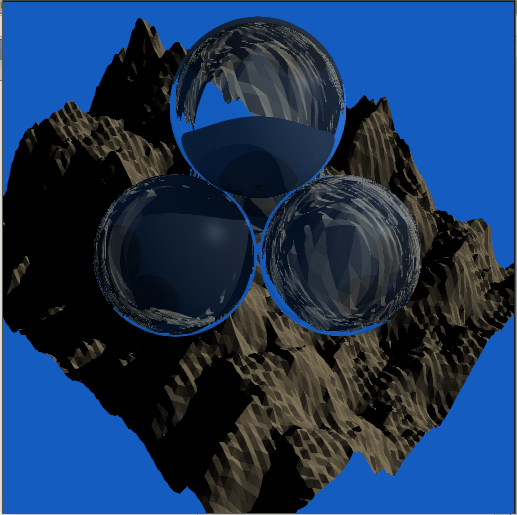
\includegraphics[width=\linewidth]{mount_very_high.png}
            \caption{mount\_very\_high.nff}
            \label{fig:mount_very_high}
        \end{subfigure}

        \caption{Refracções}
        \label{fig:balls}
    \end{figure}

    \begin{figure}[h!]
        \centering
        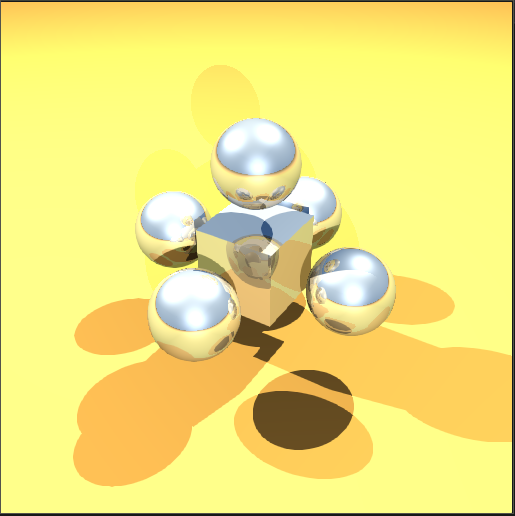
\includegraphics[width=.2\linewidth]{aabb.png}
        \caption{aabb.nff}
        \label{fig:aabb}
    \end{figure}

\end{document}